\documentclass[a4paper,12pt]{article}

\usepackage[top=3cm, bottom=2cm, left=3cm, right=2cm]{geometry}
\usepackage[utf8]{inputenc}
\usepackage[portuguese]{babel}
\usepackage{booktabs}
\usepackage{multirow}
\usepackage{multicol}
\usepackage{graphicx}
\usepackage{longtable}
\usepackage{verbatim}
\usepackage{minted}

\usepackage{float}
\floatstyle{ruled}
\newfloat{program}{thp}{lop}
\floatname{program}{Script}

\title{Tecnologias de Base de Dados\\
\Large{Trabalho de SQL3}}

\author{André Fernandes (ei03107) \and Pedro Batista (ext10392)}

\begin{document}

\maketitle

\section{Modelo de classes}

	A figura \ref{fig:classes} apresenta o modelo de classes que serviu para modelar o problema proposto. Este modelo comporta algumas alterações pequenas ao problema original, nomeadamente:

	\begin{itemize}
		\item O relaxamento da restrição do número de moradas permitidas. 	
		\item Adição de um campo de título no tópico para servir de identificação do tópico ao utilizador (alias).  
	\end{itemize}

	Relativamente às decisões efectuadas para a construção do modelo de classes da  figura \ref{fig:classes} temos:

	\begin{itemize}
		\item A encapsulação do conceito de período de tempo numa classe pois o conceito aparece repetido no calendário e no período de repetição das mensagens do mesmo.
		\item A hierarquia das categorias foi modelada através de uma relação entre categorias com o nome de ``pai''. 
	\end{itemize}

	\begin{figure}[htp]
		\begin{center}
			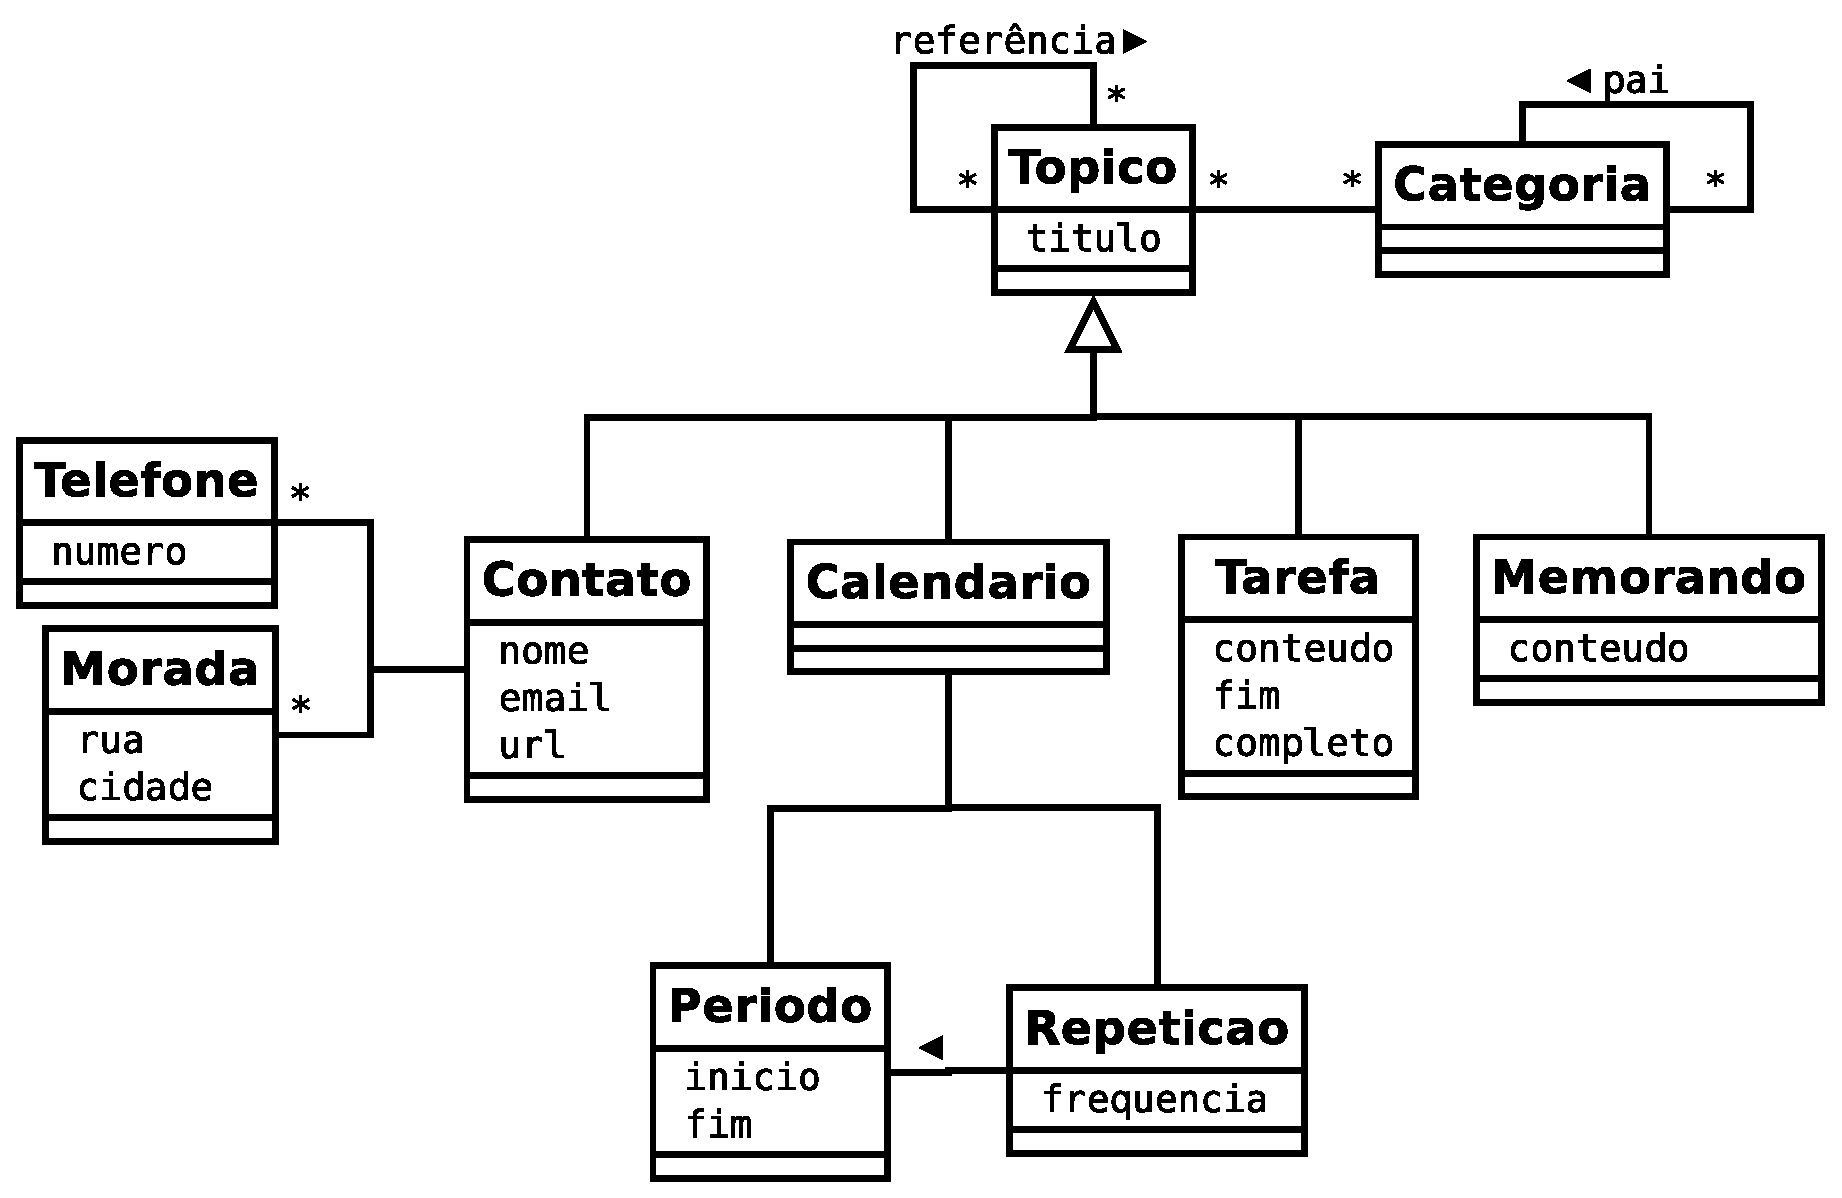
\includegraphics[height=300pt]{uml}
		\end{center}
		\caption{Modelo de classes.}
		\label{fig:classes}
	\end{figure}

\section{Modelo relacional}

	A seguir apresenta-se as tabelas que iriam ser criadas caso fossemos utilizar um modelo relacional usual.

	Nesse caso seria preciso criar uma tabela para cada tipo de dados. Com colunas com chaves primárias de outras tabelas no caso de haver uma relação de um-para-um como no caso da relação entre calendário e repetição. Ou no caso da relação muitos-para-um como na relação de telefone e contato. E seria ainda preciso criar tabelas extra para as relações muitos-para-muitos das relações entre tópicos e entre tópicos e categorias.

	\begin{multicols}{2}

		\begin{tabular}{|c|l|} \hline
			\multicolumn{2}{|c|}{TOPICO} \\ \hline
			Codigo & Tipo \\ \hline
			id & INTEGER \\
			titulo & VARCHAR(25) \\
			alteracao & DATETIME \\
			tipo & VARCHAR(11) \\
			tipo\_id & INTEGER \\ \hline
		\end{tabular}
		
		\begin{tabular}{|c|l|} \hline
			\multicolumn{2}{|c|}{REFERENCIA\_TOPICO} \\ \hline
			Codigo & Tipo \\ \hline
			de\_topico\_id  & INTEGER \\
			para\_topico\_id & INTEGER \\ \hline
		\end{tabular}
		
		\begin{tabular}{|c|l|} \hline
			\multicolumn{2}{|c|}{CATEGORIA} \\ \hline
			Codigo & Tipo \\ \hline
			id & INTEGER \\
			nome & VARCHAR(25) \\
			categoria\_pai\_id & INTEGER \\ \hline
		\end{tabular}
			
		\begin{tabular}{|c|l|} \hline
			\multicolumn{2}{|c|}{TOPICO\_CATEGORIA} \\ \hline
			Codigo & Tipo \\ \hline
			topico\_id  & INTEGER \\
			categoria\_id & INTEGER \\ \hline
		\end{tabular}
				
		\begin{tabular}{|c|l|} \hline
			\multicolumn{2}{|c|}{CONTATO} \\ \hline
			Codigo & Tipo \\ \hline
			id & INTEGER \\
			nome & VARCHAR(100) \\ 
			email & VARCHAR(100) \\
			url & VARCHAR(200) \\ \hline
		\end{tabular}
		
		\begin{tabular}{|c|l|} \hline
			\multicolumn{2}{|c|}{CALENDARIO} \\ \hline
			Codigo & Tipo \\ \hline
			id & INTEGER \\
			periodo\_id & INTEGER \\ 
			repeticao\_id & INTEGER \\ \hline
		\end{tabular}
		
		\begin{tabular}{|c|l|} \hline
			\multicolumn{2}{|c|}{TAREFA} \\ \hline
			Codigo & Tipo \\ \hline
			id & INTEGER \\
			fim & DATETIME \\ 
			completo & VARCHAR(19) \\
			conteudo & VARCHAR(255) \\ \hline
		\end{tabular}

		\begin{tabular}{|c|l|} \hline
			\multicolumn{2}{|c|}{MEMORANDO} \\ \hline
			Codigo & Tipo \\ \hline
			id & INTEGER \\
			conteudo & VARCHAR(255) \\ \hline
		\end{tabular}

		\begin{tabular}{|c|l|} \hline
			\multicolumn{2}{|c|}{TELEFONE} \\ \hline
			Codigo & Tipo \\ \hline
			id & INTEGER \\
			numero & VARCHAR(25) \\
			contato\_id & INTEGER \\ \hline
		\end{tabular}
		
		\begin{tabular}{|c|l|} \hline
			\multicolumn{2}{|c|}{MORADA} \\ \hline
			Codigo & Tipo \\ \hline
			id & INTEGER \\
			rua & VARCHAR(100) \\
			cidade & VARCHAR(50) \\
			contato\_id & INTEGER \\ \hline
		\end{tabular}

		\begin{tabular}{|c|l|} \hline
			\multicolumn{2}{|c|}{PERIODO} \\ \hline
			Codigo & Tipo \\ \hline
			id & INTEGER \\
			inicio & DATETIME \\
			fim & DATETIME \\ \hline
		\end{tabular}
		
		\begin{tabular}{|c|l|} \hline
			\multicolumn{2}{|c|}{REPETICAO} \\ \hline
			Codigo & Tipo \\ \hline
			id & INTEGER \\
			frequencia & VARCHAR(7) \\
			periodo\_id & INTEGER \\ \hline
		\end{tabular}

	\end{multicols}

\section{Modelo objecto-relacional}

	Os tipos de dados adicionados à base de dados foram praticamente transpostos do modelo de classes e estão apresentados a seguir. 
	
	Apenas temos de realçar:

	\begin{itemize}
		\item O campo pai das categorias é uma referência para uma Categoria.
		\item Os tópicos tem um conjunto de referências Categoria e um conjunto de referências Tópico.
		\item Os contatos contêm conjuntos de Morada e Telefone.
		\item E as repetições e calendários integram tipos de Período. 
	\end{itemize}

	\begin{multicols}{2}

		\begin{tabular}{|c|l|} \hline
			\multirow{4}{*}{TOPICO}
			& titulo VARCHAR(25) \\
			& alteracao DATETIME \\ 
			& categorias S\_CATEGORIA \\
			& referencias S\_TOPICO\\ \hline 
		\end{tabular}
		
		\begin{tabular}{|c|l|} \hline
			\multirow{4}{*}{CONTATO}
			& nome VARCHAR(25) \\
			& telefones S\_TELEFONE \\ 
			& moradas S\_MORADA \\
			& email VARCHAR(100) \\ 
			& url VARCHAR(200) \\ \hline 
		\end{tabular}
		
		\begin{tabular}{|c|l|} \hline
			\multirow{2}{*}{CALENDARIO}
			& p PERIODO \\
			& r REPETICAO \\ \hline 
		\end{tabular}
		
		\begin{tabular}{|c|l|} \hline
			\multirow{3}{*}{TAREFA}
			& fim DATETIME \\
			& completo VARCHAR(1) \\ 
			& conteudo VARCHAR(255) \\ \hline 
		\end{tabular}
		
		\begin{tabular}{|c|l|} \hline
			MEMO & fim DATETIME \\ \hline
		\end{tabular}
		
		\begin{tabular}{|c|l|} \hline
			\multirow{2}{*}{CATEGORIA}
			& nome VARCHAR(25) \\
			& pai REF CATEGORIA \\ \hline 
		\end{tabular}
		
		\begin{tabular}{|c|l|} \hline
			\multirow{2}{*}{REPETICAO}
			& frequencia VARCHAR(7) \\
			& p PERIODO \\ \hline 
		\end{tabular}
		
		\begin{tabular}{|c|l|} \hline
			\multirow{2}{*}{PERIODO}
			& inicio DATETIME \\
			& fim DATETIME \\ \hline 
		\end{tabular}
		
		\begin{tabular}{|c|l|} \hline
			\multirow{2}{*}{MORADA}
			& rua VARCHAR(100) \\
			& cidade VARCHAR(50) \\ \hline 
		\end{tabular}
		
		\begin{tabular}{|c|l|} \hline
			TELEFONE & numero VARCHAR(25) \\ \hline 
		\end{tabular}
		
		\begin{tabular}{|c|l|} \hline
			S\_CATEGORIA & SET(REF CATEGORIA) \\ \hline
		\end{tabular}
		
		\begin{tabular}{|c|l|} \hline
			S\_TOPICO & SET(REF TOPICO) \\ \hline
		\end{tabular}
		
		\begin{tabular}{|c|l|} \hline
			S\_MORADA & SET(MORADA) \\ \hline
		\end{tabular}
		
		\begin{tabular}{|c|l|} \hline
			S\_TELEFONE & SET(TELEFONE) \\ \hline
		\end{tabular}

	\end{multicols}

	Relativamente à solução do modelo relacional, a utilização de tipos permite que o programador trabalhe a um mais alto nível de abstração. Por exemplo, é muito simples inserir um contato com várias moradas através dos contrutores de CONTATO, S\_MORADA e MORADA. 

	E existem ainda mais vantagens nas relações muitos-para-muitos porque não é necessário criar uma tabela específica para a relação. Como se pode reparar pela relação entre tópicos e categorias e ainda nas referências entre tópicos.  

\section{Interrogações}

	Apesar das respostas às perguntas estarem presentes nesta secção, o código relativo à criação de tipos, criação de tabelas, e preenchimento de dados irá estar presente no anexo do relatório.

%	A única resposta que não estará completamente respondida nesta secção é a Questão 4, uma vez que a resposta a esta pergunta envolve a descrição de uma série de procedimentos e funções PL/SQL. No entanto, todo este código também esta presente em anexo.

\subsection{Questão 1}

	\emph{Quantos tópicos há, em cada aplicação, para cada categoria?}\\

	\inputminted{sql}{1.sql}

\subsection{Questão 2}

	\emph{Quais os tópicos que têm referências a pelo menos três pessoas?}\\

	\inputminted{sql}{2.sql}

\subsection{Questão 3}

	\emph{Qual o dia mais preenchido do mês, sendo que as sobreposições só contam uma vez?	}\\

	A resposta a esta questão envolve uma série de procedimentos e funções em PL/SQL que estão apresentados em Anexo.

	Optámos por desenvolver um algoritmo suficientemente genérico para lidar com qualquer calendarização ao invés de utilizar um que usasse uma granularidade de 5 minutos. A única decisão que tivemos que fazer prende-se com a precisão e foi decidir quando ocorre a transição entre dias. Na qual optou-se por usar segundos, isto é, um dia acaba as '23:59:59' e o seguinte começa as '00:00:00'.

	Outro aspecto importante da implementação é o facto de ser suficientemente robusta para que o cálculo das horas ocupadas de um dia terem em conta os calendários, que tenham começado em qualquer altura no passado e se estendem até esse dia. E é ainda capaz de nesse cálculo ter em conta as calendarizações resultantes de repetições de um calendário.

	Para testar a nossa implementação basta:
	
	\inputminted{sql}{3.sql}

\subsection{Questão 4}

	\emph{Quais os tópicos complexos que têm referências para tópicos de todas as aplicações?}\\

	\inputminted{sql}{4.sql}

\subsection{Questão C}

	\emph{Como procederia para saber qual a profundidade da hierarquia de categorias?}\\

	\inputminted{sql}{C.sql}


\newpage 
\section{Anexo - Código}

	%\begin{minted}{sql}
	%	SELECT * FROM buh;
	%\end{minted}

	\inputminted{sql}{sql3.sql}

\end{document}
